\documentclass[11pt]{article}
\usepackage{hdtt2020}
\usepackage{newpxmath}
\usepackage{newpxtext}
\usepackage{tikz}

\newcommand{\coerce}{\ensuremath{\textnormal{transp}}}
\newcommand{\Glue}{\ensuremath{\texttt{Glue}}}
\newcommand{\glue}{\ensuremath{\texttt{glue}}}
\newcommand{\unglue}{\ensuremath{\texttt{unglue}}}
\newcommand{\hcomp}{\ensuremath{\textnormal{hcomp}}}
\newcommand{\hfilltt}{\ensuremath{\textnormal{hfill}}}
\newcommand{\transptt}{\ensuremath{\textnormal{transp}}}
\newcommand{\U}{\ensuremath{\mathcal{U}}}

\title{CSCI 8980 Higher-Dimensional Type Theory\\ Lecture Notes}
\author{Jack Perisich, Dawn Michaelson}
\date{April 14, 2020}

\begin{document}

\maketitle


\section{Universes}
Three main issues arise when discussing universes in cubical type theory: coercion in universes, composition in universes, and univalence. \\

For some $A : \U$ and constraint $\phi$, then: $$ \coerce^i \; \U \; \phi \; A \equiv A $$
This means that we can just do nothing, similar to how we handled coercion for inductive types. 

The other two issues are more involved and require the introduction of the '\texttt{Glue}' types. \texttt{Glue} types are similar to other compositions, except that the walls are eqivalences instead of paths. The \texttt{Glue} type for some $A : \U$ and $\phi \vdash E : T \simeq A$ is written as: $$ \Glue \; [\phi \mapsto (T, E)] \; A$$ This can also be thought of as using univalence to get a path from the equivalence $E$ and then composing a new type using that path as the walls in the composition.

\section{Glue Types}
Since \texttt{Glue} types are types, they must be defined in the same way as all other types. The formation rule for a \texttt{Glue} type is:
\begin{prooftree*}
	\hypo{A : \U}
	\hypo{\phi \vdash T : \U}
	\hypo{\phi \vdash E : T \simeq A}
	\infer3{\Glue \; [\phi \mapsto (T, E)] \; A : \U \; [\phi \mapsto T]}
\end{prooftree*}
This means that if we have a type $A : \U$ and this type is equivalent to the partial type $T$ under the constraint $\phi$, we can construct a \texttt{Glue} type that is judgementally equal to the type $T$ under the constraint $\phi$. \\

The introduction rule defines the only constructor for the \texttt{Glue} type called '\texttt{glue}'. It is as follows:
\begin{prooftree*}
	\hypo{\phi \vdash t : T}
	\hypo{a : A \; [\phi \mapsto \text{fst} \; E \; t]}
	\infer2{\glue \; [\phi \mapsto t] \; a : (\Glue \; [\phi \mapsto (T, E)] \; A) \; [\phi \mapsto t]}
\end{prooftree*}
This rule takes two arguments: an element of the partial type $T$ and a total element of the type $A$ which agrees with the image of $t$ judgementally. \\

The eliminator for a \texttt{Glue} type is called '\texttt{unglue}' and returns the base type that is equivalent to the partial element. More formally:
\begin{prooftree*}
	\hypo{u : \Glue \; [\phi \mapsto (T,E)] \; A}
	\infer1{\unglue \; [\phi \mapsto E] \; u : A \; [\phi \mapsto \text{fst} \; E \; u]}
\end{prooftree*}

Applying the eliminator to the constructor and the constructor to the eliminator will work as expected. In the first case: $$\unglue \; [\phi \mapsto E] \; (\glue \; [\phi \mapsto t] \; a) \equiv a : A$$ and in the second case: $$u \equiv \glue \; [\phi \mapsto u] \; (\unglue \; [\phi \mapsto E] \; u) : \Glue \; [\phi \mapsto (T, E)] \; A$$
\newpage

\section{Composition of Glue Types}
We will also need to define the Kan operators for the \texttt{Glue} types. For the homogeneous composition we can construct a 3-cube where the top face has the first \texttt{Glue} type on the front edge (M) and the second \texttt{Glue} type as the left wall (N). This means that the corresponding edges on the bottom face will have the total elements retrieved by applying the eliminator on the two \texttt{Glue} types. To get the result of the homogeneous composition, we need to call hfill on M (1). This will give a line that we can use for the right wall of the top face. By applying \texttt{unglue} to this result, we can get the entire right face (2), at which point we have enough information to perform homogeneous composition on the bottom face of the cube (3). This will give us a \texttt{Glue} type in the back face, since we have the two points on top as well as the bottom edge. 

\begin{center}
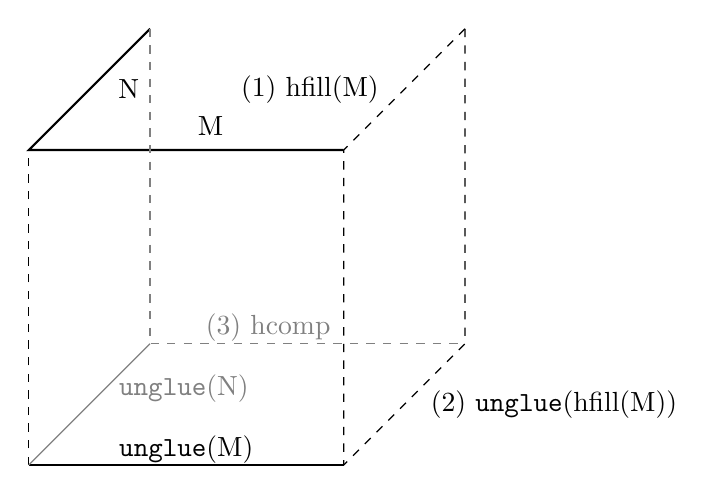
\begin{tikzpicture}
  \draw[thick](0,4,0)--(0,4,4)--(4,4,4);
  \draw[thick](4,0,4)--(0,0,4);
  \draw[dashed](4,4,0)--(4,4,4)--(4,0,4);
  \draw[dashed](4,4,0)--(4,0,0)--(4,0,4);
  \draw[dashed](0,0,4)--(0,4,4);
  \draw[gray,dashed](0,4,0)--(0,0,0)--(4,0,0);
  \draw[gray](0,0,0)--(0,0,4);
  
  \draw(2, 4, 3.2) node{\text{M}};
  \draw(0.5, 4, 2) node{\text{N}};
  \draw(2, 0.2, 4) node{\unglue(\text{M})};
  \draw[gray](1.2, 0.2, 2) node{\unglue(\text{N})};
  \draw(2.8, 4, 2) node{(1) \hfilltt(\text{M})};
  \draw(5.9, 0, 2) node{(2) \unglue(\hfilltt(\text{M}))};
  \draw[gray](1.5, 0.2, 0) node{(3) \hcomp};
\end{tikzpicture}
\end{center}

\section{Coercion of Glue Types}
To perform coercion, we will take the \texttt{Glue} type being coerced and make it the front edge of the top face of a 3-cube. Yet again, the corresponding edge on the bottom face will be the partial element resulting from applying the eliminator to the \texttt{Glue} type. This will give us the front face of the cube. We will use this to try and get the back face of the cube, which will represent coercion applied to the \texttt{Glue} type. First, we will coerce both sides of the front edge of the top face to the other side of the face using transp-fill (1). Since this gives us the left and right edge of the top face, we can project these down to the bottom face which will give us the left and right faces of the cube. We then have enough information to perform heterogeneous composition on the bottom face of the cube to get the back edge of the bottom face (2). We can then use the inverse function to get the corresponding edge on the top face (3). 

\begin{center}
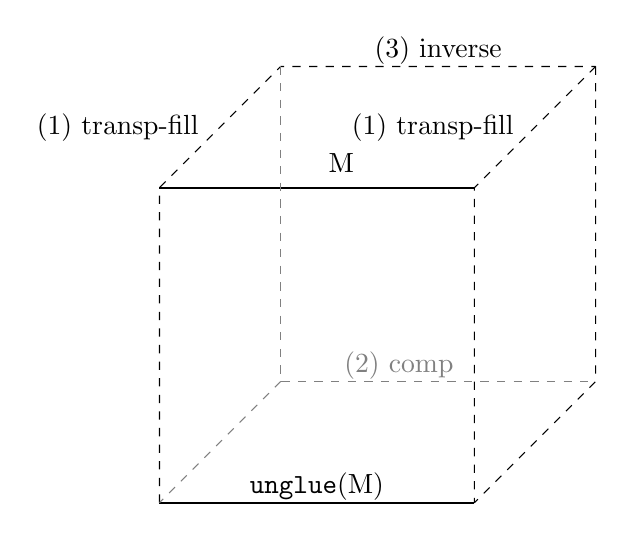
\begin{tikzpicture}
  \draw[thick](0,4,4)--(4,4,4);
  \draw[thick](4,0,4)--(0,0,4);
  \draw[dashed](4,4,0)--(4,4,4)--(4,0,4);
  \draw[dashed](4,4,0)--(4,0,0)--(4,0,4);
  \draw[dashed](0,0,4)--(0,4,4)--(0,4,0)--(4,4,0);
  \draw[gray,dashed](0,4,0)--(0,0,0)--(4,0,0);
  \draw[gray,dashed](0,0,0)--(0,0,4);
  
  \draw(2, 4, 3.2) node{\text{M}};
  \draw(-1.3, 4, 2) node{(1) \text{transp-fill}};
  \draw(2, 0.2, 4) node{\unglue(\text{M})};
  \draw(2.7, 4, 2) node{(1) \text{transp-fill}};
  \draw[gray](1.5, 0.2, 0) node{(2) \text{comp}};
  \draw(2, 4.2, 0) node{(3) \text{inverse}};
\end{tikzpicture}
\end{center}

However, the projection of this edge may not agree with the bottom edge judgementally, so the last step in the algorithm requires us to fix the back edge of the bottom face. We can get a viable bottom edge by applying homogeneous composition to this edge (4). This will fix the bottom edge and give us the back face which finishes the coercion. 

\begin{center}
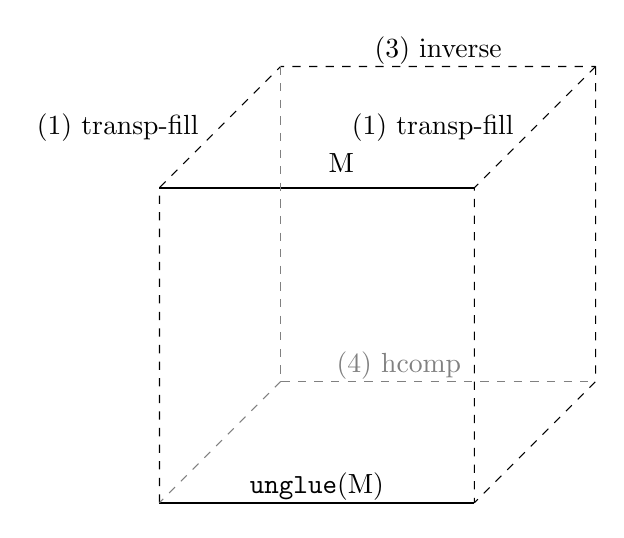
\begin{tikzpicture}
  \draw[thick](0,4,4)--(4,4,4);
  \draw[thick](4,0,4)--(0,0,4);
  \draw[dashed](4,4,0)--(4,4,4)--(4,0,4);
  \draw[dashed](4,4,0)--(4,0,0)--(4,0,4);
  \draw[dashed](0,0,4)--(0,4,4)--(0,4,0)--(4,4,0);
  \draw[gray,dashed](0,4,0)--(0,0,0)--(4,0,0);
  \draw[gray,dashed](0,0,0)--(0,0,4);
  
  \draw(2, 4, 3.2) node{\text{M}};
  \draw(-1.3, 4, 2) node{(1) \text{transp-fill}};
  \draw(2, 0.2, 4) node{\unglue(\text{M})};
  \draw(2.7, 4, 2) node{(1) \text{transp-fill}};
  \draw[gray](1.5, 0.2, 0) node{(4) \hcomp};
  \draw(2, 4.2, 0) node{(3) \text{inverse}};
\end{tikzpicture}
\end{center}

\section{Univalence}
Finally, to implement univalence, we can set the bottom of the box to one of the two types (B), put the equivalence (E) on the left wall, and set the right wall to be the identity equivalence of the bottom element. This will give a path in the top edge between the two types as follows: $$\transptt^i \; (\text{ua}(E)@i) \; 0 \; a \equiv \text{id} \;(\transptt^i \; B \; 0 \; (\text{fst} \; E \; a))$$ Note that coercion along the constant type is not an identity function. This condition (called regularity) is difficult to include due to univalence.

\end{document}

